\documentclass[a4paper,12pt, final]{report}
\usepackage{graphicx}
\usepackage{url}
%\usepackage[nomain,acronym,xindy,toc]{glossaries} % nomain, if you define glossaries in a file, and you use \include{INP-00-glossary}
%\makeglossaries
%\usepackage[xindy]{imakeidx}
%\makeindex
%\usepackage[section]{placeins}
\renewcommand\bibname{References}
\usepackage[utf8]{inputenc}
%\usepackage{algorithm2e}
%\usepackage{wrapfig}
\usepackage{epsfig}
%\usepackage{hyperref}
\usepackage[hidelinks]{hyperref} % To Hide the box around links
\renewcommand\bibname{References}
%\usepackage{algorithm2e}
\usepackage{color}
\usepackage{textcomp}
\usepackage{acronym}
\usepackage[top=0.5in, bottom=1in, left=1in, right=1in]{geometry}
\usepackage{xcolor}
\definecolor{dark-red}{rgb}{0.4,0.15,0.15}
\definecolor{dark-blue}{rgb}{0.15,0.15,0.4}
\definecolor{medium-blue}{rgb}{0,0,0.5}

\newcommand{\BigO}[1]{\ensuremath{\operatorname{O}\bigl(#1\bigr)}}
\parindent 8pt
\begin{document}
    \thispagestyle{empty}
    \vspace*{1cm}
    
{
    \centering
    \textbf{\LARGE Hardware Security}\\
    \vspace{1.20cm}
    %\it
    %\vspace{.5cm}
    %\rm
    \textbf{\large Seminar Monthly Report - September}\\
    \vspace{1cm}
    {Submitted in partial fulfillment of the requirements}\\
    \vspace{0.25cm}
    {for the course}\\
    \vspace{1cm}
    \textbf{EE694}\\
    \vspace{1.50cm}
    {by}\\
    \vspace{0.20cm}
    \textbf{\large Kalind Karia}\\
    \vspace{0.25cm}
    \textbf{\large (Roll No. 213076001)}\\
    \vspace{1.8cm}
    {Under the guidance of}\\
    \vspace{0.20cm}
    \textbf{\large Prof. Virendra Singh}\\
    \vspace{0.30cm}
    \vspace{1.450cm}
    
    \begin{figure}[htb]
        \begin{center}
            
\includegraphics[height=1.5in,width=1.5in]{images/iitblogo.png}
        \end{center}
    \end{figure}

    {\textbf{Department of Electrical Engineering}}\\
    {\textbf{Indian Institute of Technology Bombay}}\\[10pt]
    {\textbf{September 2022}}
 
}
 
\renewcommand{\abstractname}{Acknowledgement}
\begin{abstract}
    I express my gratitude to my guide Prof. Virendra Singh for providing me the opportunity to work on this topic. 
    \\\\
    \\\\
    \\\\
    Kalind Karia\\
    Electrical Engineering\\
    IIT Bombay\\\
\end{abstract}


\clearpage 
% \renewcommand{\abstractname}{Abstract} 
% \abstract{XX.}

\tableofcontents
    \addcontentsline{toc}{chapter}{\listfigurename}
    \listoffigures
%  \printglossaries

\chapter{Introduction}
The CIA triad is widely used information security model designed to guide policies for information security. This triad suits well for information security in computer architecture as well. The initials stand for three principles in information security:
\begin{itemize}
    \item Confidentiality: Only authorized party should be able to access or modify the data being computed.
    \item Integrity: Data being computed should maintain its correct state.
    \item Availability: The computed data should be readily accessible to authorized parties.
\end{itemize}

\section{Need for virtual memory}
Operating System (OS) loads program's code, data, stack, heap, etc. from disk to memory (DRAM) upon its execution. When such multiple active programs or processes are time-sharing the CPU, each process's memory must be present in DRAM. The processes memory cannot be placed contiguously in DRAM, since it will waste much of the DRAM space when one of the process terminates and the new process wants large space than the one which terminated. Thus OS provides virtualization of memory by allocating virtual address space to each process. Every process assumes that it has access to large space of memory. Memory Management Unit (MMU) performs the translation from virtual address to physical address space.

\section{Paging and Page Table}
So, a process executes in its private virtual address space composed of pages (fixed size chunks), each representing a contiguous range of addresses. Thus, CPU issues load or store to process's virtual addresses. OS divides the virtual address space into fixed size pages and physical memory into frames. Each page is mapped to an arbitrary frame in physical memory. Page table stores mappings from virtual page number to physical frame number for a process. MMU has access to the page table and uses it to translate virtual address to physical address. OS tells the hardware (MMU) the base (starting address) and bound (total size of process memory) values.

\section{Translation Look-aside Buffer (TLB)}
Page table is an array of page table entries (PTE), one per virtual page or process. When CPU requests a load for code/data using virtual address, MMU first accesses memory (DRAM) to read page table entry, then translates virtual address to physical address and then accesses the memory (DRAM) again to fetch the process code/data. Thus paging adds overhead to memory access. Solution is to cache the recently used page table entries in the Translation Look-aside Buffer (TLB). So, MMU first looks for an entry in TLB. If TLB hit, then physical address can be directly used. If TLB miss, then MMU performs additional memory accesses to "walk" the page table. Hence, TLB misses are expensive. TLB is completely managed by hardware and not OS. TLB is a scarce processor resource with a small number of entries. Large pages use the TLB more efficiently due to fewer entries.

\section{Need for Caches and Cache Hierarchy}
A memory access to DRAM typically takes 100s of cycles. Minimizing costly DRAM accesses is critical for performance of a processor. This is due to main memory or DRAM being slower as compared to fast processors. To overcome this, smaller but faster memories called caches are used to reduce the effective memory access time. Caches store frequently used instruction or data so that their access by the processor is faster. The processor request for data first reaches the cache, if data is available in cache, it is called a cache hit. If the requested data is not available in cache, it results into cache miss and the request goes to main memory to fetch the required data.

To improve the performance further, modern processors have hierarchy of caches. Higher-level caches, that are closer to the processor are smaller but faster than lower-level caches that are closer to main memory. Each core typically has three private top-level caches, L1i (Level-1 instruction), L1d (Level-1 data) and L2 (Level-2). Last-level Cache (LLC) is shared among all the cores of a multi-core chip and is a unified cache i.e., it holds both data and instructions. More the cache levels adds more levels of access in memory hierarchy. But this has a trade-off between access time and latency. Total latency of access through multi-level caches must be less than DRAM latency.

A memory access request first accesses the L1 cache, and on a miss, the request is sent down the hierarchy until it hits the lower-level cache or accesses main memory. Figure 1.1 shows the system model of mutli-core processor.

\begin{figure}[h]
    \centering
    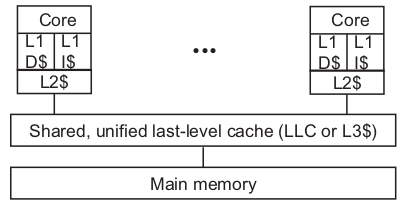
\includegraphics[scale=0.7]{images/multi_core_system_model.png}
    \caption{System model of multi-core processor \cite{prime_probe_llc}}
    % \label{fig:my_label}
\end{figure}

\section{Cache access}
Caches are organized in fixed-size \textit{lines} or \textit{blocks}. A typical line size \textit{B} is 64 bytes. The $\log_{2}B$ lowest-order bits of the virtual address, called the \textit{line offset} or \textit{block offset} are used to locate data in the cache line. On memory access, complete line or block is brought into the cache from main memory.

Caches are usually set-associative, i.e. organized as \textit{S} sets of \textit{W} lines each, called a \textit{W-way set-associative} cache. As shown in Figure 1.2, upon memory access, the \textit{set index} field of the address, $\log_{2}S$ bits starting from bit $\log_{2}B$ is used to locate a \textit{cache set}. The remaining higher-order bits are used as a \textit{tag} for each cache line. Once the cache set is located, the tag field is matched against the tag of the \textit{W} lines in the set to identify if one of the cache lines is a cache hit.

\begin{figure}[h]
    \centering
    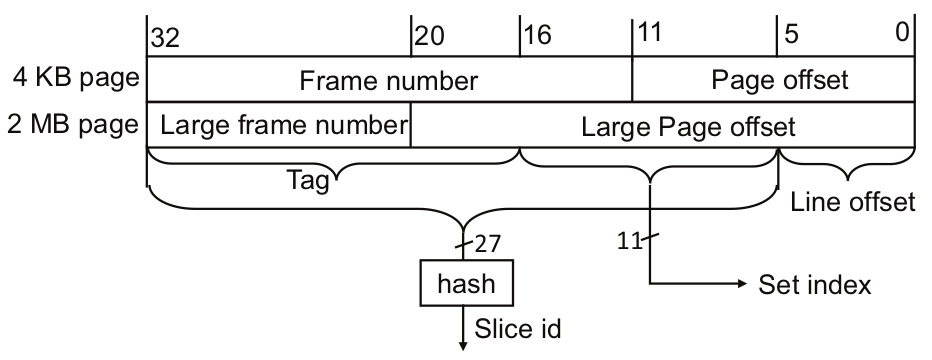
\includegraphics[scale=0.4]{images/sliced_cache.png}
    \caption{Virtual address mapping for a cache \cite{prime_probe_llc}}
    % \label{fig:my_label}
\end{figure}

If an access misses in the cache, data is brought from lower-level cache or main memory and one cache line is evicted to free a slot for the newly fetched cache line. The cache's \textit{replacement policy} determines the line to be evicted. Typically, least-recently-used (LRU) policy is used.

\section{Cache Inclusiveness}
Multi-level caches have defined relationship between different levels of cache based on whether the content of one cache is present in other levels of caches.

\begin{itemize}
    \item If all blocks in the higher level cache are also present in the lower level cache, then the lower level cache is said to be \textit{inclusive} of the higher level cache.
    \item If the lower level cache contains only blocks that are not present in the higher level cache, then the lower level cache is said to be \textit{exclusive} of the higher level cache.
    \item If the contents of the lower level cache are neither strictly inclusive nor exclusive of the higher level cache, then it is called \textit{non-inclusive} cache.
\end{itemize}

Modern Intel processors like Sandy Bridge use more complex architecture for the LLC, to improve its performance. The LLC is divided into per-core \textit{slices}, which are connected via a ring bus. Cores can access these slices concurrently, and the ring bus ensures that each core can access the full LLC. A hash function is used to map the address to the \textit{slide id} as shown in Figure 1.2.

\section{Is Page sharing vulnerable to attack?}
OS shares identical memory pages between processes to reduce the memory footprint, for e.g. in case of shared libraries. Sharing of pages requires the need for maintaining isolation between non-trusting processes, and to achieve this \textit{copy-on-write} or \textit{read-only} semantics are followed. This semantics does not stop one process to read cached data.

Lets take an example, processes P1 and P2 running on different cores have a copy of shared library (lets say of GnuPG) in their respective memory footprint. When P1 accesses a function of GnuPG, it will face cache miss initially and bring the corresponding data to LLC and its private cache (due to cache inclusiveness). This access would be slow due to number of cache misses. Now, when P2 accesses the same function, since the data is already present in the LLC (shared between both processes) the access time will be shorter than P1. In this way, one process can influence the execution time of another process. P2 can also use this knowledge of timing difference to extract information from P1. This is called a \textit{side-channel} attack since the attacker uses the side effects of micro-architecture to mount an attack.

\section{Speculative Execution}
In out-of-order execution, often processor reaches a conditional branch instruction whose direction depends on the preceding instructions which are not yet completed. Instead of being idle until the conditional branch completes execution, processor makes a guess of a path, saves a checkpoint of its current state i.e. registers and memory, and speculatively executes the instructions on that path. When the conditional branch reaches ROB head, it is resolved and the correctness of processor's guess is determined. The instructions executed speculatively are committed if the CPU's prediction turns out to be correct, this provides greater advantage over idle waiting. However, if the prediction turns out to be incorrect, it reverts the computations of speculative execution and resumes from the instruction on correct path after the guess. But the effects in micro-architecture state is not reverted such as cache. Thus the instructions that are executed incorrectly due to mis-prediction but leave behind traces in micro-architecture are called \textit{transient instructions}. The state change in micro-architecture (after reverting back to the saved checkpoint) is vulnerable to leaking sensitive information to the adversary.

\chapter{Literature Survey}
Page sharing in case of shared library can influence the execution time of a process since the shared data or code has been fetched by another process during first access into the cache (LLC in case of cross-core or cross-VM and L1, L2 in case of single-core). This timing difference can be tracked by attacker process to determine the access pattern of the victim process. It assists in leaking secret data via side-channel. This idea is the basis of the Flush + Reload attack \cite{flush_reload}. It is demonstrated by extracting private encryption keys used in square-and-multiply exponentiation algorithm of GnuPG program.

Flush + Reload attack is limited by the requirement of page sharing. Prime + Probe attack \cite{prime_probe_llc} overcomes this shortcoming by relying on (i) inclusive nature of LLC and (ii) use of large pages. It describes an algorithm to determine an eviction set consisting of memory lines which is accessed by victim as well. They too have demonstrated the attack on GnuPG program leaking the secret key of victim. It is shown that the attack is possible in modern processors with sliced caches without reverse engineering the hash function. This is supported by large pages used by hypervisor for improved performance.

Spectre attack \cite{spectre} comes under different class of attack. It exploits the features of modern processors that help boosting the CPU performance such as branch predictor and speculative execution. Speculative execution has a side-effect on micro-architecture that its state is not reverted back when CPU resumes execution of the correct path. The incorrect execution of instructions was previously assumed to be safe. This paper shows how the branch predictor can be mis-trained forcing the victim process to speculatively execute transient instructions and leak sensitive information in the caches (a micro-architecture). It has multiple variants based on the method of achieving speculative execution and the method used to leak information. It is a serious threat to processors from Intel, ARM, AMD which have speculative execution capabilities. This attack requires shared memory between victim and attacker.

\chapter{Review}

% \section{Flush + Reload attack}

% \subsection{Summary}

% \subsection{Strengths}

% \subsection{Weaknesses}

% \subsection{Opportunities}

\section{Last-Level Cache Side-Channel Attacks are Practical}

\subsection{Summary}

\hspace{5pt} In this paper \cite{prime_probe_llc}, the authors present an effective implementation of Prime + Probe side-channel attack on LLC. They have demonstrated the attack on cross-core, cross-VM and measured the capacity of the covert channel created.

% \vspace{5pt}
The work presented in the paper adapts the Prime + Probe technique for practical LLC attacks by exploiting hardware features such as:

\begin{enumerate}
    \item inclusive caches (outside control of the cloud provider)
    \item large page mappings (controllable and usually enabled in VMM for better performance)
\end{enumerate}

Only other assumption made is that the attacker and victim are co-hosted on the same processor.

% Major contributions of the work:
% \begin{enumerate}
%     \item asynchronous Prime + Probe attack on LLC that does not require sharing of cores or memory between attacker and victim and does not exploit VMM weaknesses.
%     \item develops two techniques for efficient attack:
%     \begin{itemize}
%         \item algorithm for attacker to probe exactly one cache set without the knowledge of virtual-address mapping
%         \item use temporal access patterns to identify victim's security-critical accesses.
%     \end{itemize}
%     \item achieves the measurable bandwidth of cross-VM covert timing channel as high as 1.2 Mb/s.
% \end{enumerate}

Their LLC-based cross-core, cross-VM attack is based on Prime + Probe \cite{prime_probe_l1} where the attacker learns which cache set is accessed by the victim VM.

Attacker, \verb|A|, runs a spy process to monitor cache usage of victim, \verb|V| as follows:
\begin{enumerate}
    \item Prime: \verb|A| fills selected cache sets with its own code/data
    \item Idle: \verb|A| waits for a pre-configured time while \verb|V| executes and utilizes the cache
    \item Probe: \verb|A| again accesses the selected cache sets and measures the time to load each set
\end{enumerate}

If \verb|A| finds that the access latency is more during Probe, then \verb|V| would have evicted some of \verb|A|'s lines during Idle. Conversely, if the access latency is less then \verb|V| has not used or evicted the selected cache sets of \verb|A|.

Challenges for efficient Prime + Probe attack on LLC and how were they overcome are listed below:
\begin{enumerate}
    \item Visibility of victim's activity at LLC
    \begin{itemize}
        \item LLC has less visibility into victim's memory activity than L1 since L1 and L2 will satisfy most of the victim's memory accesses.
        \item If manipulation to LLC by attacker does not change the state of L1, L2 (private to victim VM), then victim's accesses will never reach LLC and will be hidden from the attacker.
        \item It is overcomed by leveraging cache inclusiveness that helps replacing victim's data from complete cache hierarchy without accessing victim's private caches.
    \end{itemize}
    
    \item Infeasibility of priming and probing whole LLC
    \begin{itemize}
        \item Since LLC is very large in size, it is not feasible to access every set.
        \item Hence very few cache sets relevant to victim's accesses are determined and only these sets are monitored during prime and probe.
    \end{itemize}
    
    \item Identify cache sets relevant to victim's accesses without probing the whole LLC
    \begin{itemize}
        \item Attacker has no idea of the victim's virtual address space and has no control on its mapping.
        \item Solution is to scan entire LLC monitoring one cache set at a time, look for temporal access patterns that are relevant to victim's accesses. These patterns are specific to the algorithm used.
        \item An eviction set is constructed which is then primed and probed.
    \end{itemize}
\end{enumerate}

The attack is demonstrated by extracting key from (a) secret-dependent execution paths (Square-and-Multiply modular exponentiation) and (b) secret-dependent data access patterns (Sliding-window modular exponentiation) on the GnuPG tool. The core idea of the attack is to monitor the use of squaring operations. It is shown that the exponent can be recovered by observing the time between subsequent squarings.

\subsection{Strengths}

\begin{itemize}
    \item Prime + Probe attack is an efficient asynchronous LLC-based cross-core, cross-VM attack i.e. attacker and victim only have LLC in common that is shared among all the cores of a multi-core processor.
    \item This attack removes the requirement of shared memory and libraries between attacker and victim process upon which the Flush + Reload attack primarily depends.
    \item This attack is possible even in modern Intel processors which have sliced cache.
    \item Much higher bandwidth of up to 1.2 Mb/s is achieved.
\end{itemize}

\subsection{Weaknesses}

\begin{itemize}
    \item Attack depends on the inclusiveness of caches. If the caches are not inclusive, then priming and probing of eviction set will have no effect on victim's local caches and the victim's access will be hidden from the attacker.
    \item Large page mappings in VMM helps in construction of eviction set without the knowledge of virtual addresses relevant to victim's accesses. Assumption is made that VMM uses large frames to map guest physical memory.
    \item If the victim executes a fixed-window (or constant-time) exponentiation algorithm, then the notion of monitoring time between subsequent accesses fails and it is impossible to mount the attack.
\end{itemize}

\subsection{Opportunities}

\begin{itemize}
    \item The attack is not tested in a noisy environment or in a real cloud settings. One can experiment the attack in such situations to measure the effects of noise.
    \item One can experiment the attack's working without the dependence on large pages (but with reduced efficiency).
\end{itemize}

\section{Spectre Attack: Exploiting Speculative Execution}

\subsection{Summary}
CPUs use speculative execution and branch predictors to maximize their performance. Speculative execution involves CPU making a incorrect guess to the future execution paths and execute instructions on these paths. CPU eventually reverts or squashes the incorrect speculative execution results to the state before the guess was made; these incorrectly executed instructions that leave behind micro-architectural traces are called transient instructions.

This paper \cite{spectre} exploits the speculative execution feature in influencing a victim process to execute transient instructions which otherwise would haven't occurred in correct program execution. Attacker can decide which transient instructions should be speculatively executed in order to leak secret information from the victim process.

Spectre attack has multiple variants based on the method of inducing erroneous speculative execution and of leaking data via covert channel.
\begin{itemize}
    \item Exploiting Conditional Branches
    \begin{itemize}
        \item Attacker mistrains the CPU's branch predictor by initially providing valid inputs. During exploit phase, it provides malicious inputs to load victim's secret data into cache.
        \item When CPU discovers the erroneous execution and reverts the changes, since changes to cache state are not reverted, the attacker can access the data from victim's address space.
    \end{itemize}
    
    \item Exploiting Indirect Branches
    \begin{itemize}
        \item Attacker trains the Branch Target Buffer (BTB) to mispredict a branch from an indirect branch to a location where transient instructions are present, resulting in their speculative execution.
        \item This leaks the victim's sensitive information via cache side channel.
    \end{itemize}
\end{itemize}

\subsection{Strengths}
\begin{itemize}
    \item This attack violates the process or memory isolation boundaries as well as sandboxing. Processors from Intel, ARM and AMD are vulnerable to this attack due to their speculative execution capabilities.
    \item The only assumption made is that speculatively executed instructions can read from memory that the victim process could access normally.
    \item Preventing speculative execution would significantly degrade the performance of the processor and will require fixes to processor design and ISA, hence this solution cannot provide immediate fix to Spectre attack.
\end{itemize}

\subsection{Weaknesses}
\begin{itemize}
    \item Victim and attacker must share memory address space in order to leak the victim's data via side-channel.
    \item Victim and attacker processes must run on same core (if the architecture provides individual branch predictor for each core) since branch predictor of victim is mistrained resulting into speculative execution of transient instructions.
\end{itemize}

% \subsection{Opportunities}

\chapter{Conclusion}
Micro-architectural attacks are a class of different types of attacks categorized into Cache Timing, Branch Prediction, Speculative, Row Hammer types of attacks, etc. These attacks have been used to break cryptographic algorithms, containerization, process or memory isolation boundaries, etc.

Cache Timing attacks are based on the memory access patterns observed in the victim's process to leak the sensitive data via side-channel into the cache. Flush + Reload, Prime + Probe are good examples for the same that can be mounted cross-core, cross-VM with high resolution. Such attacks are not possible on algorithms which have fixed-window (or constant-time) implementation.

Spectre attack is based on the features in modern processors i.e. speculative execution and branch predictors. It violates the isolation boundary between processes and cannot be easily fixed since the solution will require changes to ISA and processor design.

Broadly, there are trade-offs between security and performance. The long-standing focus on maximizing performance needs to be shifted to increased performance with security. The mitigations for these attacks should be optimized for more than one attack and prevent the chance of occurrence of a new attack.

\bibliographystyle{ieeetr}
\bibliography{thesisTemplate}{}

\end{document}
